\appendix
\UnnumberedChapter{PHỤ LỤC}

\section*{Phụ lục 1. Hình ảnh giao diện hệ thống}

Phụ lục này trình bày một số giao diện chính của hệ thống Secure Chat System with Cryptographic Security nhằm minh họa quá trình xây dựng và kết quả đạt được sau khi hoàn thành đề tài.

\begin{itemize}
    \item Giao diện đăng ký tài khoản (Register).
    \begin{figure}[H]
    \centering
    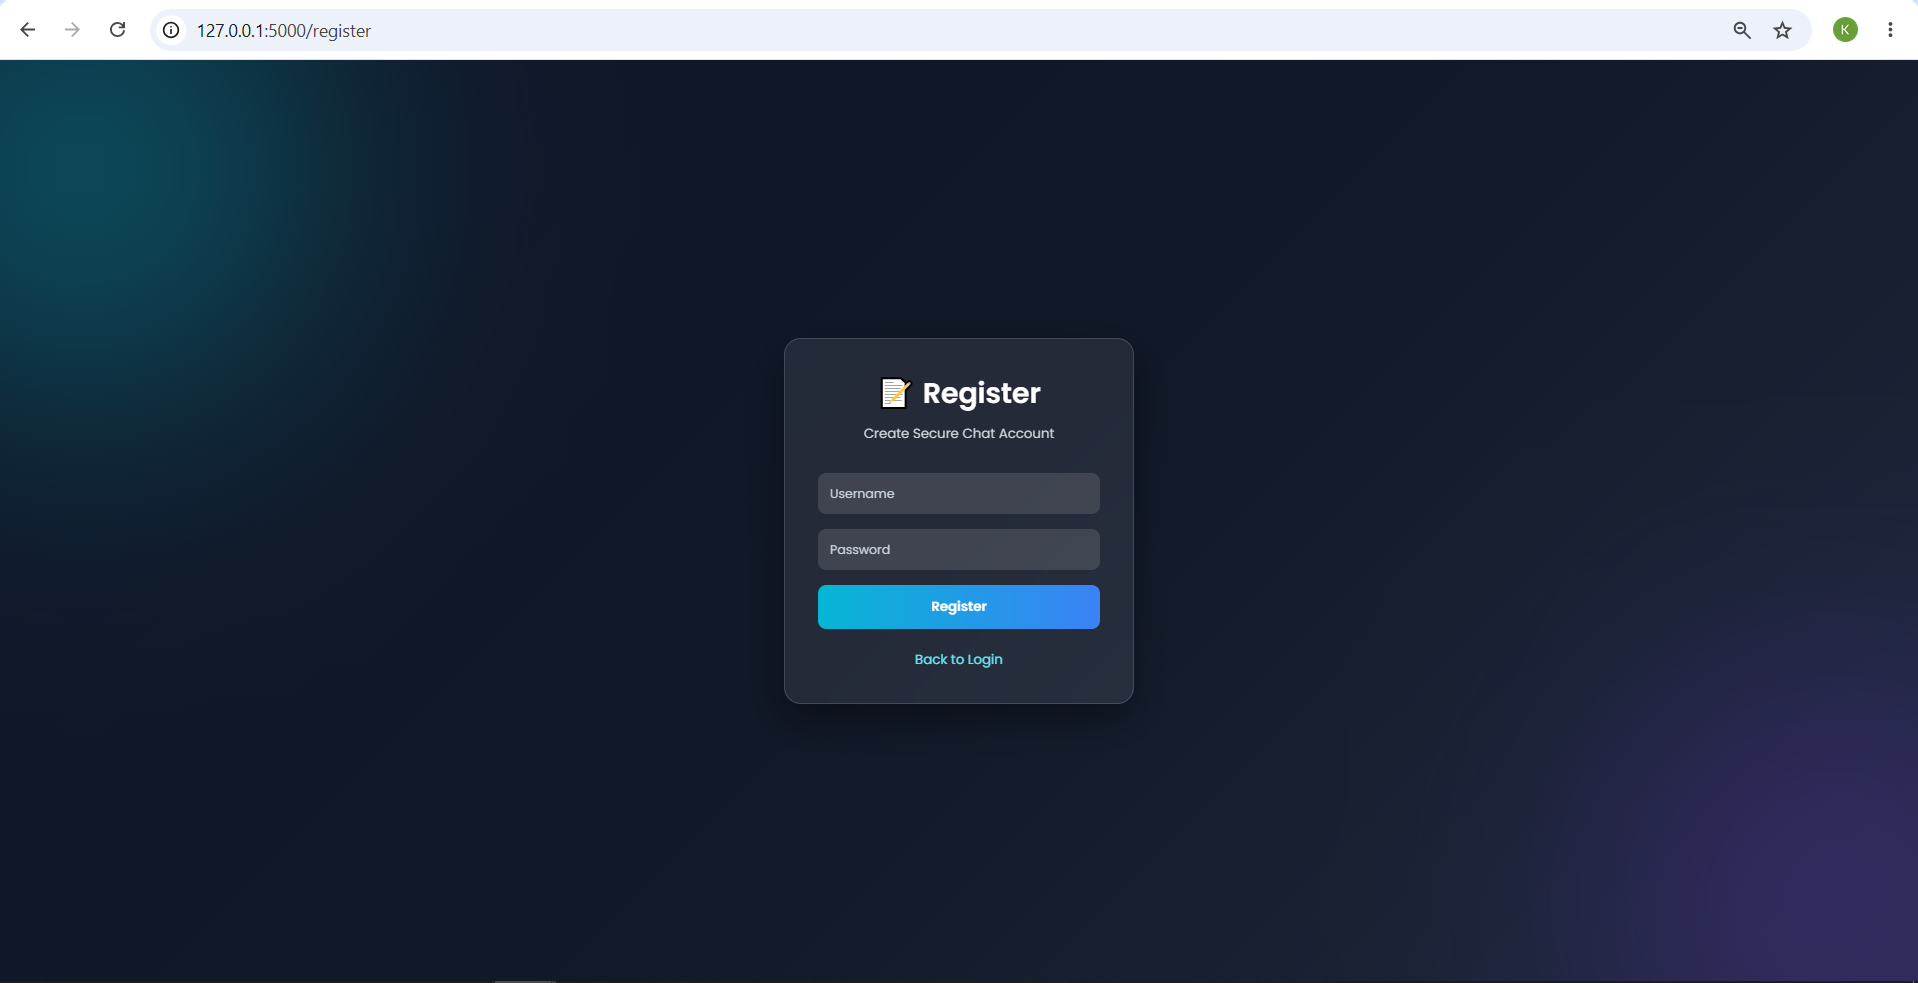
\includegraphics[width=0.9\textwidth]{images/register.png}
    \caption{Giao diện đăng ký tài khoản}
    \label{fig:register}
    \Nguon{Trần Khiêm}
    \end{figure}
    \item Giao diện đăng nhập hệ thống (Login).
    \begin{figure}[H]
    \centering
    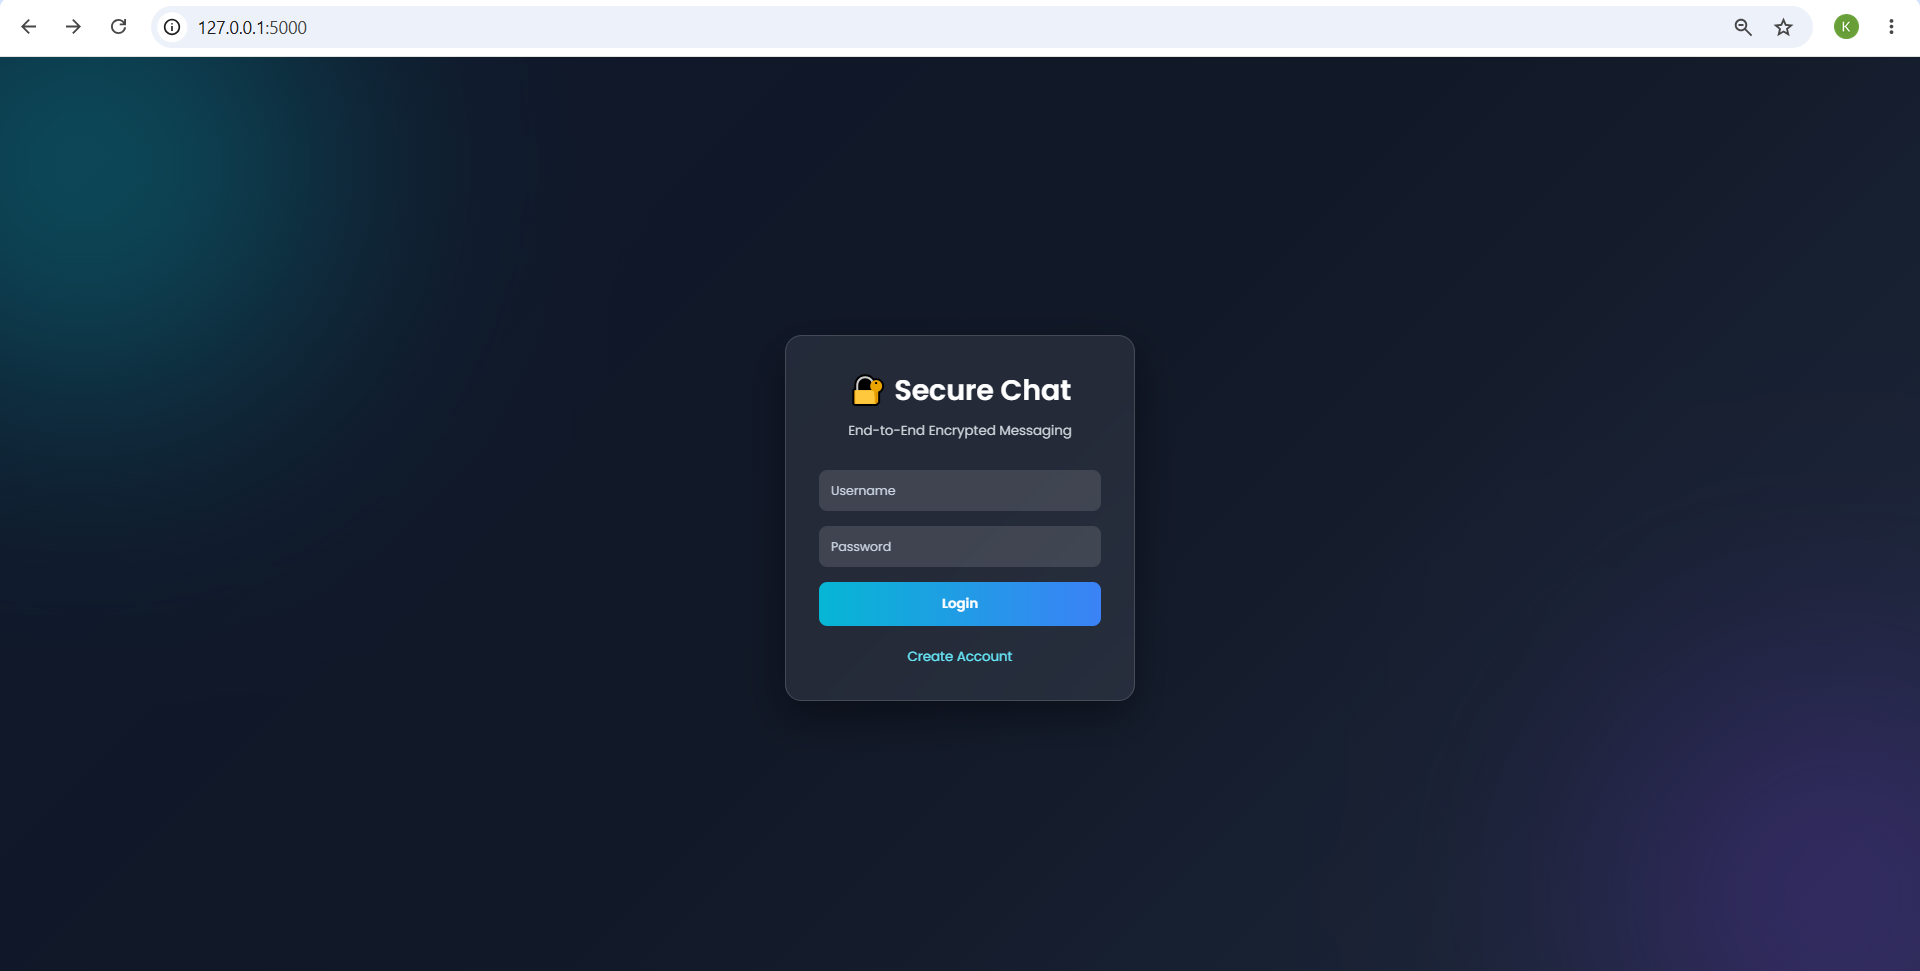
\includegraphics[width=0.9\textwidth]{images/login.png}
    \caption{Giao diện đăng nhập}
    \label{fig:login}
    \Nguon{Trần Khiêm}
    \end{figure}
    \item Giao diện nhắn tin thời gian thực (Chat).
    \begin{figure}[H]
    \centering
    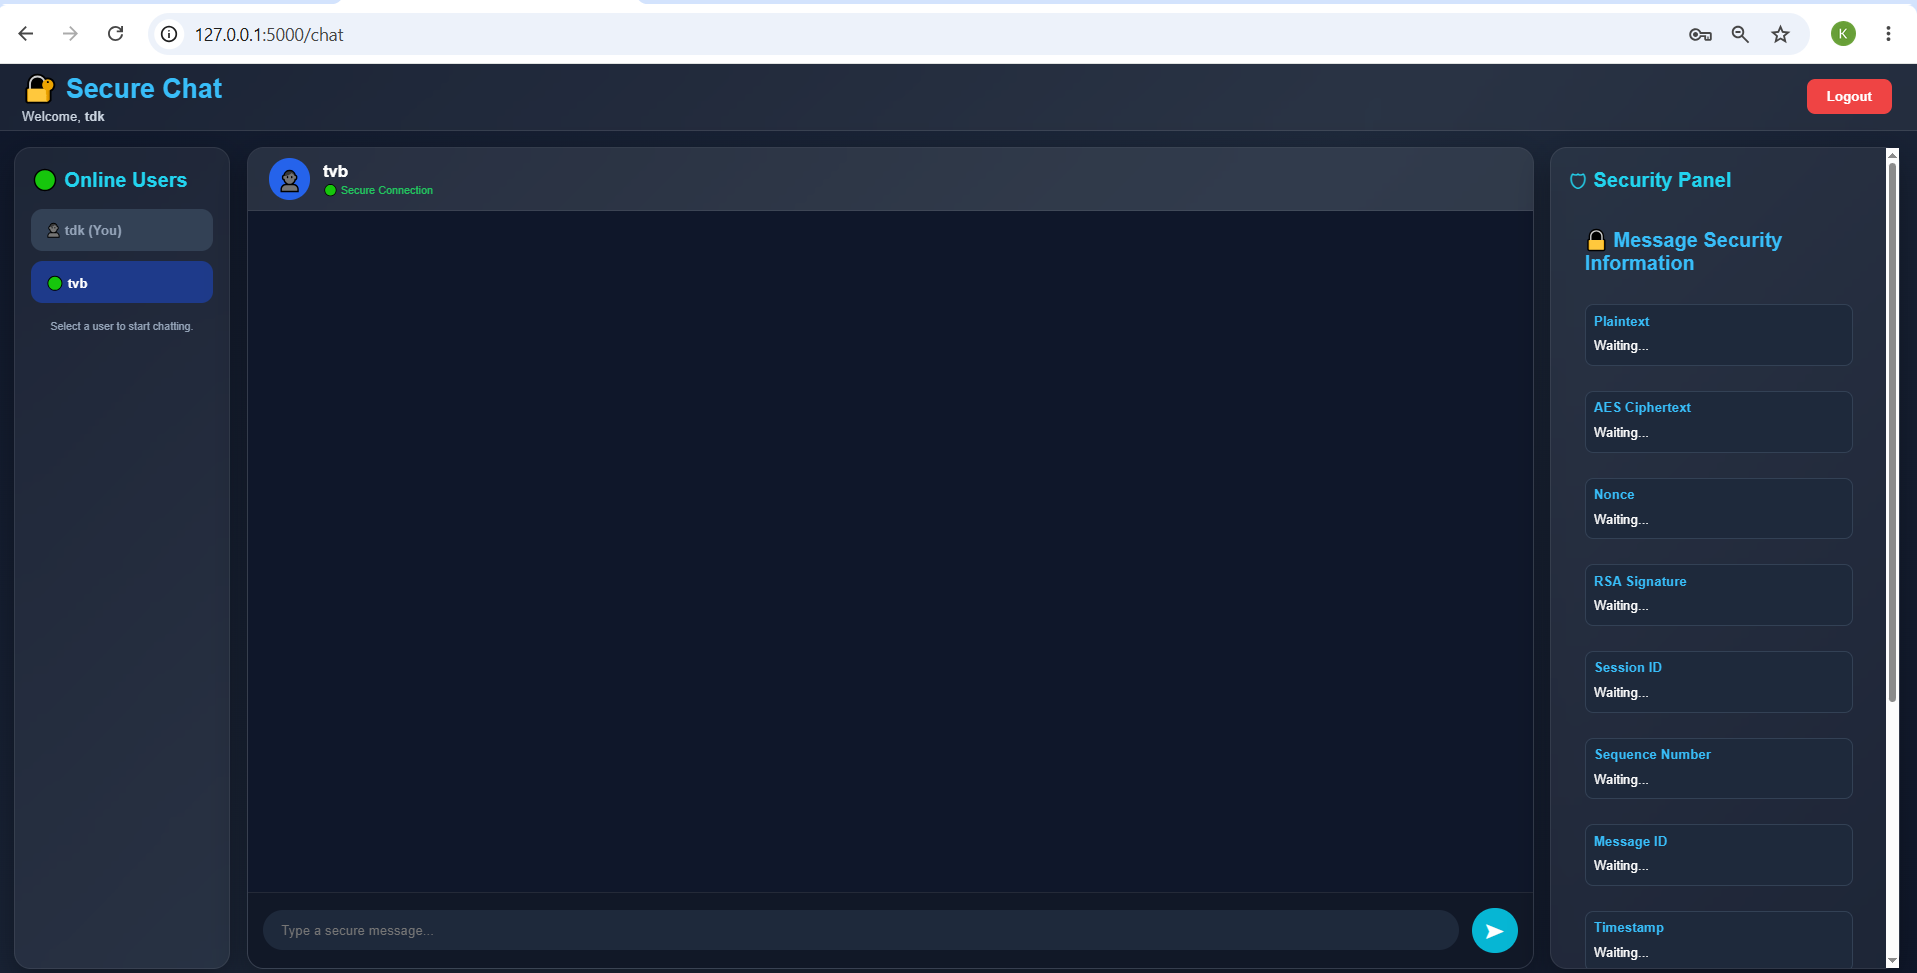
\includegraphics[width=0.9\textwidth]{images/chat.png}
    \caption{Giao diện nhắn tin thời gian thực}
    \label{fig:chat}
    \Nguon{Trần Khiêm}
    \end{figure}
    \item Giao diện Security Information hiển thị các thông tin bảo mật của từng gói tin.
    \begin{figure}[H]
    \centering
    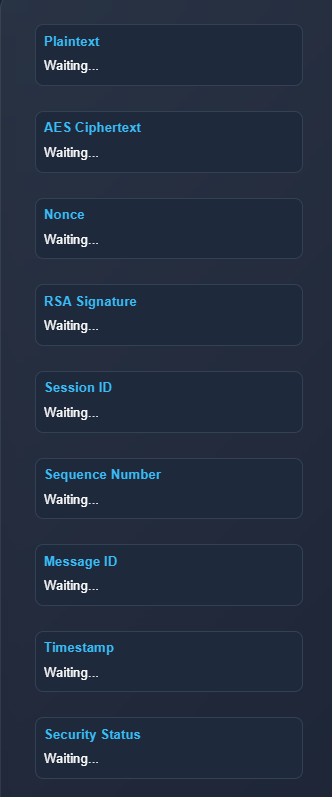
\includegraphics[height=0.75\textheight,keepaspectratio]{images/security.png}
    \caption{Giao diện Security Information}
    \label{fig:security}
    \Nguon{Trần Khiêm}
    \end{figure}
    \item Giao diện mô phỏng các cuộc tấn công như Modify Ciphertext, Replay Attack, Wrong Session Key, Fake Sender và Modify Sequence Number.
    \begin{figure}[H]
    \centering
    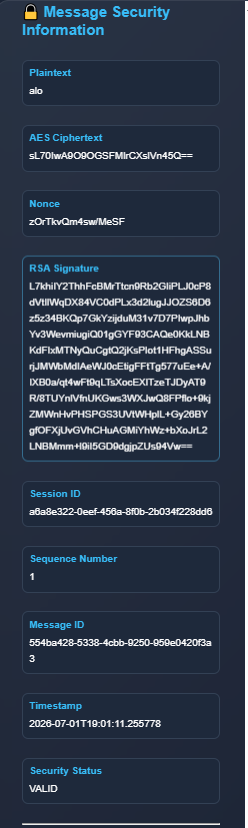
\includegraphics[height=0.75\textheight,keepaspectratio]{images/security1.png}
    \caption{Tiếp tục giao diện Security Information}
    \label{fig:security1}
    \Nguon{Trần Khiêm}
    \end{figure}
\end{itemize}

\section*{Phụ lục 2. Cấu trúc dự án}

Dự án được tổ chức theo cấu trúc thư mục nhằm thuận tiện cho việc phát triển và bảo trì hệ thống.

\begin{itemize}
    \item app.py: Chương trình chính khởi động Web Server.
    \item routes/: Xử lý các yêu cầu HTTP.
    \item templates/: Chứa các giao diện HTML.
    \item static/: Chứa CSS, JavaScript và các tài nguyên tĩnh.
    \item crypto/: Cài đặt các thuật toán RSA-OAEP, AES-GCM và RSA-PSS.
    \item security/: Xử lý Replay Detector, Session Manager và Session Key Rotation.
    \item database/: Quản lý dữ liệu người dùng và phiên làm việc.
\end{itemize}

\section*{Phụ lục 3. Môi trường phát triển}

Hệ thống được xây dựng và kiểm thử trong môi trường sau:

\begin{itemize}
    \item Hệ điều hành: Windows 10/11.
    \item Python 3.12.
    \item Flask.
    \item Flask-SocketIO.
    \item Cryptography Library.
    \item Visual Studio Code.
    \item Git và GitHub.
\end{itemize}

\section*{Phụ lục 4. Liên kết dự án}

Nếu được phép công bố, có thể bổ sung các liên kết sau:

\begin{itemize}
    \item Link GitHub của dự án.
    \item Video demo hệ thống.
    \item Tài liệu hướng dẫn sử dụng.
    \item Slide thuyết trình.
\end{itemize}